
\documentclass[a4paper,twoside,twocolumn,10pt]{article}
\usepackage{abstract} % Style for abstracts in Dept. CSIS, OPU
%\usepackage{abstract4past} % Style for abstracts for the past curriculum

%%%%%%%%%% Designate packages you need %%%%%%%%%%
\usepackage[dvipdfmx]{graphicx}   %pLaTeX2e仕様(\documentstyle ->\documentclass)
\usepackage{url} % Verbatim with URL-sensitive line breaks
\usepackage{bm}
\usepackage{amsmath}
\usepackage{amsfonts}
\newcommand{\bv}[1]{\mbox{\boldmath$#1$}}
\newcommand{\argmax}{\mathop{\rm arg~max}\limits}
\newcommand{\argmin}{\mathop{\rm arg~min}\limits}
\usepackage{comment}
\usepackage{subcaption}
\usepackage{graphicx}

%%%%%%%%%% Parameters that should be customized %%%%%%%%%%
% Language (1 = Japanese, 2 = English)
\setlang{1}
% Bachelor or Master (1 = Bachelor, 2 = Master)
\setborm{1}
% Fiscal year
\setfy{2023}
% 研究室番号
\setgnum{1}
% 発表順
\setorder{4}
% Increase page number (optional)
%% \pplus{1}

% Title
\title{Masked Language Modeling を用いた\par Knowledge Graph 補完手法の提案}
% Author
\author{堀本 隆誠}
%%%%%%%%%% Parameters that should be customized (end) %%%%%%%%%%

\begin{document}
\maketitle % Insert title
\small

\section{はじめに}

近年, 人工知能技術は急速な発展を遂げている. その中で人間の知識をグラフ構造で表現する Knowledge Graph \cite{kg} が注目を集めており, 人工知能の基盤技術としてさまざまな分野で活用されている. しかし, Knowledge Graph 内の知識とそれらの関係を人手ですべて網羅するには多大なコストがかかる. この問題を解決するために Knowledge Graph 内の関係を基に含まれていない関係を自動的に補完する手法が求められている. 本研究では,言語モデルである BERT の Masked Language Modeling を用いて Knowledge Graph を補完する手法を提案して, その有効性を検証した.\par

\vspace{-1mm}
\section{要素技術}

\subsection{Knowledge Graph}

Knowledge Graph \cite{kg} とは, さまざまな知識を体系的に連結し, その関係をグラフ構造で表した知識ネットワークのことである. Knowledge Graph は, head, tail を要素に持つ entity 集合と, その entity 間の関係を表現する relation を要素に持つ relation 集合によって構成されており, (head, relation, tail) という 3 つ組構造(triple)の集合で表すことができる. \par

\vspace{-1mm}
\subsection{BERT}

Bidirectional Encoder Representations from Transformers (BERT) \cite{BERT} は, Transformer をベースとして双方向エンコーダで構成された言語モデルである. BERT は, マスクされた単語を予測する Masked Language Modeling (MLM) と 2 つの文が連続するかを分類する Next Sentence Prediction (NSP) という 2 つの手法で学習している. \par
Knowledge Graph BERT (KG-BERT) \cite{KG-BERT} は, Yao らによって提案された BERT を用いた Knowledge Graph 補完手法の 1 つである. KG-BERT では, triple を表した文 ``[CLS] head [SEP] relation [SEP] tail [SEP]" を  BERT の入力として, その triple が存在するか否かを ``[CLS]" トークンのみを利用した 2 値分類で判定している. \par

\vspace{-1mm}
\subsection{WN18RR}

WN18RR \cite{wn18rr} は, 英語の大規模な語彙データベースである WordNet から triple を自動抽出して得られたデータセット WN18 から作られており, WN18 から head と tail を入れ替えて得られる逆関係の triple を除去したデータセットとなっている. WN18RR では, entity の head, もしくは tail が ``見出し語, その説明文" の形で表される. \par

\vspace{-1mm}
\section{提案手法}

Knowledge Graph の triple における head, relation, tail をそれぞれ h, r, t とすると, Knowledge Graph 補完では triple (h, r, ?) に対して ? に入る tail を回答することで entity 間の関係性を予測する. 本研究では, BERT の MLM を fine-tuning したモデルに triple (head, relation, [MASK]) を 1 つのシーケンスとして入力して tail を予測することによる Knowledge Graph 補完手法を提案する. 

% triple を表した文 ``[CLS] head [SEP] relation [SEP] tail [SEP]" に対して, tail の見出し語を ``[MASK]" トークンに置き換えた文 ``[CLS] head [SEP] relation [SEP] [MASK], tail の説明文 [SEP]" と, その説明文を除去した文 ``[CLS] head [SEP] relation [SEP] [MASK] [SEP]" の 2 種類を入力として BERT の MLM をファインチューニングしたモデルを使用した. 学習はこの 2 種類の入力文に対して, 15\% の入力トークンを 80\% の確率で ``[MASK]" トークンに置き換え, 10\% の確率でランダムに選んだトークンに置き換え, 10\% の確率でそのままのトークンとした. つまり, tail の見出し語は必ず ``[MASK]" トークンに置き換えられている. \par

% 図
% \begin{figure}[t]
%   \centering
%   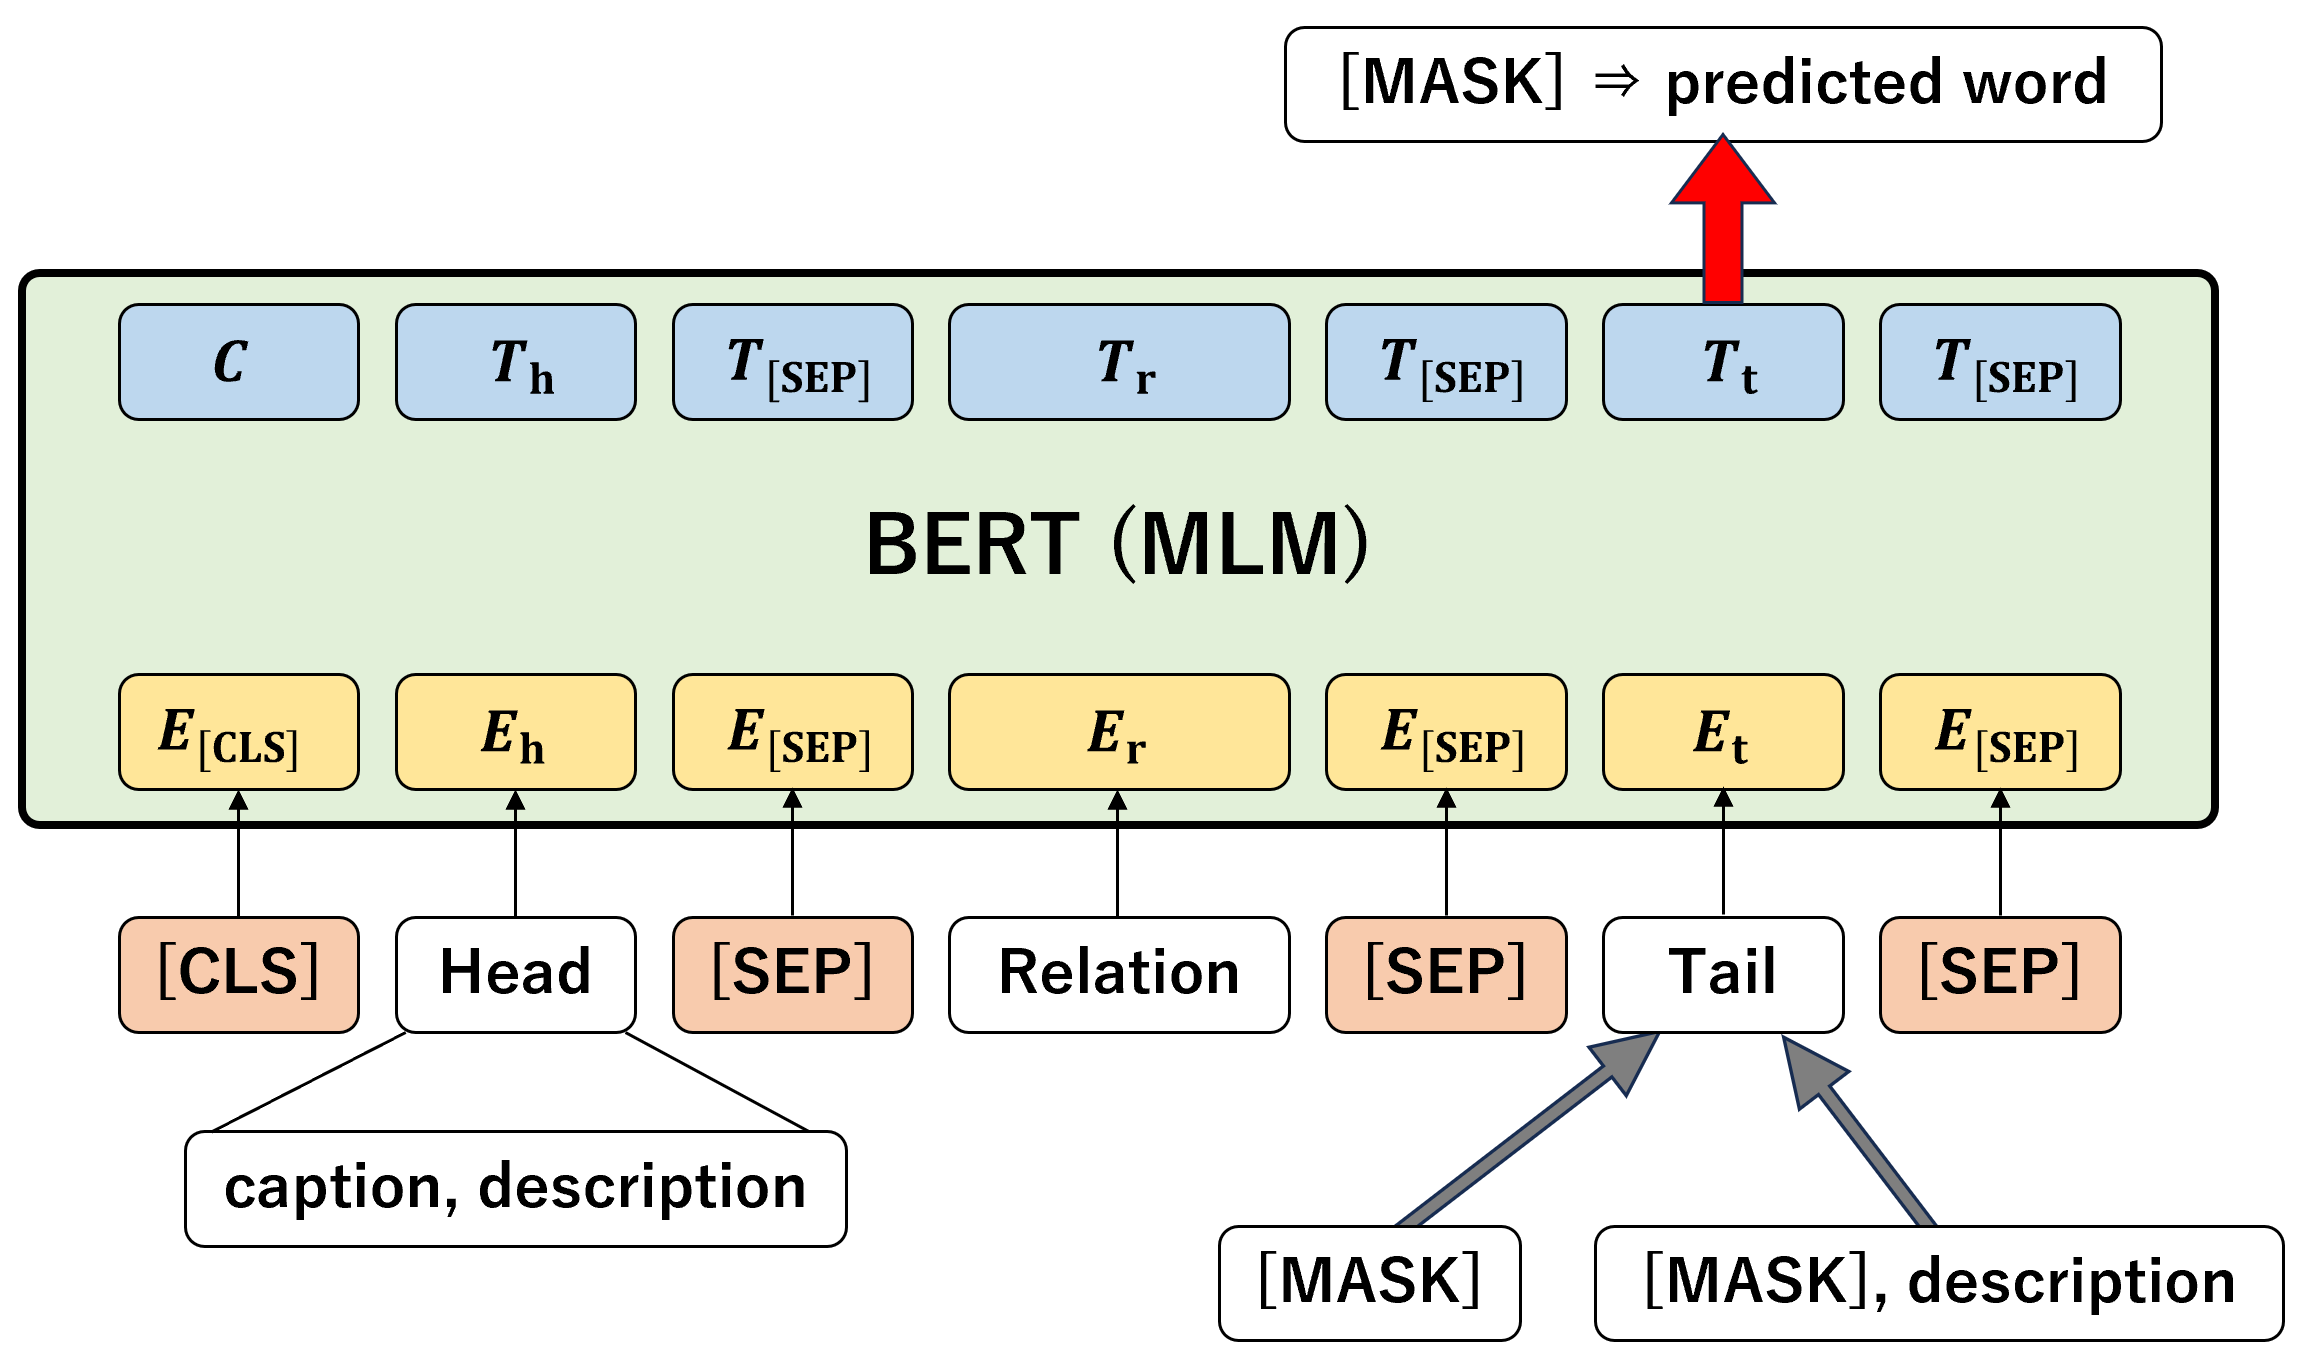
\includegraphics[width=\columnwidth]{KG-MLM.png}
%   \caption{モデルの概略図}
%   \label{KG-MLM}
% \end{figure}

\vspace{-1mm}
\section{数値実験}

BERT の MLM を fine-tuning したモデルに対して, 2 種類の入力文を用いて実験した. 実験 1 では triple ``[CLS] head [SEP] relation [SEP] tail [SEP]" に対して, tail の見出し語を ``[MASK]" トークンに置き換えた文 ``[CLS] head [SEP] relation [SEP] [MASK], tail の説明文 [SEP]" を入力文として評価した. 実験 2 では実験 1 の入力文に対して, tail の説明文を除去した文 ``[CLS] head [SEP] relation [SEP] [MASK] [SEP]" を入力文として評価した. \par
データを訓練 : 検証 : テスト = 8 : 1 : 1 に分割し, 評価には Mean Reciprocal Rank (MRR) と Hits@$k$ を使用した. 予測結果の $r$ 番目に正解があるとき, その順位 $r$ のことをランクと呼び, ${\rm |T|}$ を triple 数, $r_{i}$ を triple$_{i}$ における正解 tail のランクとすると, MRR は (\ref{MRR}) 式で表される.
\begin{equation}
    \vspace{-1mm}
    {\rm MRR} = \frac{1}{\rm |T|} \sum^{\rm |T|}_{i=1} \frac{1}{r_{i}}
    \label{MRR}
\end{equation}
Hits@$k$ は, tail 予測において上位 $k$ 個以内に正解の要素が出力されている割合を表す. 本研究では $k=1, 3, 10$ で評価した. MMR, Hits@$k$ はともに値が大きいときに推定精度が良いと判断される. \par
表 \ref{result} に KG-BERT および, 実験 1, 2 の MRR と Hits@$k$ の値を示す. 実験 1 ではすべての評価指標において KG-BERT を上回る結果が得られた. 入力に tail の説明文の情報が含まれていることにより tail の見出し語を予測できたと考えられる. 一方, 実験 2 では Hits@$1$ において KG-BERT と同程度の結果が得られたが, 他の指標においては下回る結果となった. 本実験では tail 予測の出力候補が BERT に登録されている単語すべてであるため, 出力候補を entity に限定することで精度の向上が見込まれる. \par

% 表
\begin{table}[t]
  \caption{KG-BERT と実験 1, 2 の MRR, Hits@$k$ の値}
  \label{result}
  \centering
  % \small
  \setlength{\doublerulesep}{0.4pt}
  \begin{tabular}{ccccc}\hline\hline
   & MRR & Hits@1 & Hits@3 & Hits@10 \\ \hline
   KG-BERT & $0.25$ & $12.41$ & $29.44$ & $51.85$ \\ \hline
  実験 1 & $0.546$ & $52.55$ & $56.16$ & $57.79$ \\ \hline
  実験 2 & $0.168$ & $10.94$ & $19.37$ & $27.95$ \\
  \hline\hline
  \end{tabular}
  \vspace{-3mm}
\end{table}
\vspace{-1mm}

% 表
% \begin{table}[t]
%   \caption{表のテンプレート}
%   \label{tb:sample}
%   \centering
%   % \small
%   \setlength{\doublerulesep}{0.4pt}
%   \begin{tabular}{cc}\hline\hline
%   項目 & 値 \\ \hline
%   例 & $1$ \\
%   \hline\hline
%   \end{tabular}
% \end{table}

\section{まとめと今後の課題}

本研究では, MLM を用いた 2 種類の入力文に対する tail の見出し語予測について KG-BERT と比較し, 実験 1 において KG-BERT を上回る結果が得られた. これにより MLM を用いた Knowledge Graph 補完手法の有効性が確認できた. 今後の課題として, MLM の出力候補を entity に限定したモデルの作成が挙げられる. 

\bibliographystyle{jabbrvunsrt}
\bibliography{abstract}

\end{document}
